\titleformat{\chapter}[hang]{\Huge\bfseries}{\thechapter\hsp\textcolor{gray75}{|}\hsp}{0pt}{\Huge\bfseries}
\chapter{Literature Review}
\label{chap: Lit}

\section{Prior Attempts at Solving Similar Problems}

Throughout my research of this topic, I have come across many interesting ideas from other academics and hobbyists attempting to solve similar problems as I am here. One example comes from Swartz, Gill and Muthukumarana \cite{swartz_modelling_2009} in their paper, \textit{Modelling and simulation for one-day cricket}. Another came from hobbyist, Andrew Kuo, aka. dr00bot \cite{kuo_predicting_2021} in the form of a blog post: \textit{Predicting T20 Cricket Matches With a Ball Simulation Model}. In this section, I describe the methods and findings of both papers before comparing their choice of methods and suggesting ways that I can add to and improve upon their research.

\subsection{Swartz et al.}

\subsubsection{Introduction}

In the paper, they describe their process for building a simulator for one-day international\footnote{50 overs per innings} (ODI) cricket matches. They approach this problem in a similar way to me – realising that there are a finite set of outcomes that are possible for each ball. Each of these outcomes is then assigned a probability based on historical ODI data.

A significant goal of theirs was to answer game-specific and strategy related questions. For example, ‘what would be the expected outcome of England changing the order of their third and sixth batters?’ They concluded that a simulator would be necessary to best answer these types of questions.

\subsubsection{Methods}

Their simulation proceeds as follows:
A sample is drawn from a uniform (0, 1) distribution and a no-ball/wide is assigned if the sample is less than a defined threshold. In this case, a single run is added to the batting team, and the ball is not counted as part of the limit of 300 for an ODI. Additional runs may be scored in addition to a no-ball/wide, and these are sampled from a multinomial distribution, with the same outcomes as the main one described below.

Assuming no no-ball or wide, the simulator in this experiment samples from seven possible outcomes. (Wicket, 0, 1, 2, 3, 4, 6.) Here, ‘wicket’ includes run-outs, and leg-byes and byes are included within the results of 0-6. \Cref{fig:swartz model} is taken from their paper and describes the logic nicely.

\begin{figure}[h]
    \centering
    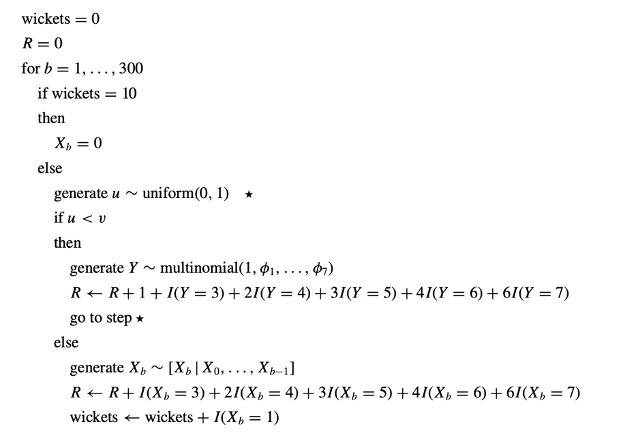
\includegraphics{images/swartz.png}
    \caption{The logic of the Swartz simulator}
    \label{fig:swartz model}
\end{figure}

Swartz et al. model each ball as a conditional distribution where the outcome of a given ball is conditional on the outcomes of the balls that have come before it. \Cref{fig:swartz2} below shows this. $X_{b}$ refers to the outcome of a given ball, where $b = 1…300$.

\begin{figure}
    \centering
    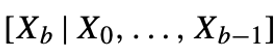
\includegraphics{images/swartz2.png}
    \caption{The conditional distribution which models each ball}
    \label{fig:swartz2}
\end{figure}

One key feature of the modelling approach applied here is the significant distinction made between first and second innings. For the first innings, only the following factors are considered as inputs to the model: the batter, bowler, number of wickets lost, and the number of balls bowled. A Bayesian latent variable model is developed to get estimates for the probabilities of the possible outcomes of $X_{b}$. This outputs probabilities based only on the batter and bowler. The output is then updated by a neat addition which is termed ‘batsman aggressiveness’. This modifies the output of the model based on the state of the game at the time (wickets remaining, balls remaining) where the batter’s willingness to take more risks will change. The model is fitted in winBUGS and 851 unknown parameters are estimated – the vast majority of these corresponding to each of the batters and bowlers in the dataset.

In the second innings, the conditional distributions also depend on the first innings score, as well as the batting team’s current score in the match. The first innings model is modified to account for these extra variables. This is done by considering the batting team’s balls and wickets remaining as combined ‘resources’ which are required to be ‘spent’ in order to score runs. This idea is taken from Duckworth and Lewis. \cite{duckworth_fair_1998} \cite{duckworth_successful_2004} A formula is devised which modifies the probability distribution calculated using the same model as in the first innings. As an example: take a scenario where the team batting second has many runs left to score to win the match, proportional to relatively few resources with which to score them. This would be a scenario where we would expect the batter to play more aggressively. This has the effect of increasing his probability of dismissal, and his probability of an optimal score of six runs. Consequently, the probability of a more typical outcome like a score of zero, or 1 run, decreases.

\subsubsection{Conclusions}

Recall that the goal of Swartz et al. in this experiment was to build a simulator to be able to answer complex game and strategy specific questions. This, in my opinion, proves to be a difficult task to assess comprehensively and with quantitative rigour. Here, we outline the steps they took to assess their model.

The first test is to see how the predictions change as the model is presented with differing scenarios. A fixed batter, A Cook in this case, is pit against two bowlers of differing abilities, G McGrath and N Hossain. As expected, Cook’s expected runs per over are smaller against McGrath than Hossain. (McGrath is widely perceived to be a superior bowler than Hossain.)

Next, these batter/bowler match-ups remained the same (Cook vs McGrath) and the game-state inputs were changed. It was discovered that on ball 1 of the innings, with all 10 wickets remaining, Cook’s expected runs per over are low at 3.7, and his probability of dismissal is also small (0.024). As we fast-forward to ball 271 (out of 300) with just 2 wickets lost – a situation that calls for significantly greater risk and aggression to be deployed by the batter – Cook’s expected runs per over do in fact increase substantially to 6.1 while his probability of dismissal also increases to 0.039. We can therefore say that the model is performing well in accounting for game-state here.

More pertinent to my investigation is their test where actual runs scored are compared to simulated runs scored across first innings. This should give us a much better representation of how this simulation-based model performs in a predictive context. For this test, 23 matches between Sri Lanka and India were selected where Sri Lanka batted first. These included 15 matches from the original training data and 8 external to the training data.  For each match, the real-life batter and bowler orders were recorded for the first innings, and the simulator was run, for 1000 times per match. The simulated runs were compared against the real-life outcomes. Results proved favourable towards the model, and these are shown in \cref{fig:swartz3} below.

\begin{figure}[h]
    \centering
    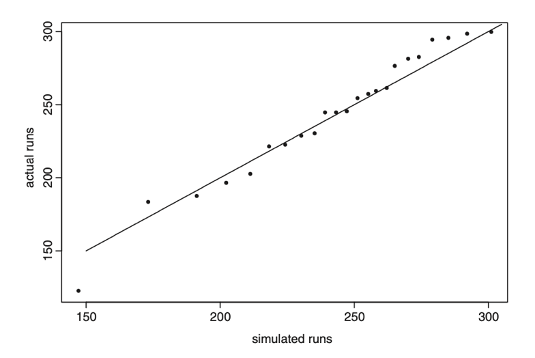
\includegraphics{images/swartz3.png}
    \caption{QQ-plot showing simulated first innings runs vs actual first innings where Sri Lanka bat against India. Taken from Swartz et al.}
    \label{fig:swartz3}
\end{figure}

The final test is to check the effectiveness of the second innings adjustment for batter aggressiveness. By considering simulated matches where Australia bat second, comparisons can be made when the simulator is set to output probabilities prior to the second innings adjustment versus including the adjustment proposed in the model description. In the simulation including the adjustment, Australia was found to have used up their full 50 overs on 8.5\% of occasions. This is in comparison to a result of 13\% when the second innings adjustment is not in operation. Comparing these benchmarks to real-life observations, we see that when Australia batted second they used up their full allocation of deliveries on 7\% of occasions. Suggesting that the model is working as intended when making these adjustments.

\subsection{dr00bot}

\subsubsection{Introduction}

The second cricket simulation idea I have taken inspiration from is a blog post by Andrew Kuo, also known as ‘dr00bot’. It was originally published on the Towards Data Science site, but can be found with no sign-in required on his website, linked here. \cite{kuo_predicting_2021}

The goal was defined by Kuo to ‘experiment with a probabilistic, bottom-up approach to modelling’. Rather like me, it seems he was curious to see how these methods would perform at prediction.

The dataset he used was comprehensive, comprising ball-by-ball information of 3651 T20 matches across 7 leagues between 2003, and 2020.

\subsubsection{Methods}

As in the Swartz paper looked at earlier, Kuo identified the crux of the project to be the generation of a probability distribution of all possible outcomes from each ball. This is termed the ball prediction model. The methods used in generating the distribution are significantly different to Swartz et al. Instead of treating the batter and bowler as factors within the model (where each batter and each bowler in the dataset has an individual parameter associated with them) Kuo inputs the bowler and batter’s respective historical statistics. This is a nice solution as it massively reduces the number of parameters required to be estimated – resulting in a model that is far less likely to suffer from overfitting. \cite{everitt_cambridge_2010} In addition, some variables related to ‘match state are also given as inputs to the model. These are innings, over, number of runs scored, number of wickets taken and first innings score (if we’re in the second innings). Each of these inputs was given to a trained feed-forward neural network model. The network comprised two dense layers each of 50 nodes, using the ReLU activation function on each node. It is a shame that more details about the intricacies of the model were not shared in the article.

The simulation engine is devised in a similar fashion to Swartz et al. above. One key difference is that wide balls are dealt with in the main simulator. Another is that there is peculiarly no mention of byes and leg byes and how they are treated. I assume that these are baked into the results corresponding to runs. This of course leads to the issue that runs for a given batsman might be ever so slightly overestimated in this model.\footnotemark{}

\footnotetext{Byes and leg-byes are recorded as extras and not attributed to the on-strike batter for the ball on which they occur.}

The simulation proceeds as follows:

A coin-toss commences the match. This decides which team bats first. The ball prediction model is then run with the current match state and relevant bowler and batter stats as inputs to the model. A random sample from the distribution output is then taken and the match state and team states are updated as determined by the sampled outcome. This process repeats until the innings is complete.

\subsubsection{Conclusions}

To test the model, Kuo took 1126 matches from his dataset and simulated them 500 times each, noting that the number of simulations was limited to 500 for reasons of computational efficiency. He compared the results of his simulations against the outcomes in the corresponding real-life games.

The first test was a crude visual comparison between simulated matches and real-life matches to check to see how well his simulations compared with real-life games from the point-of-view of realism.

\begin{figure}[hb]
    \centering
    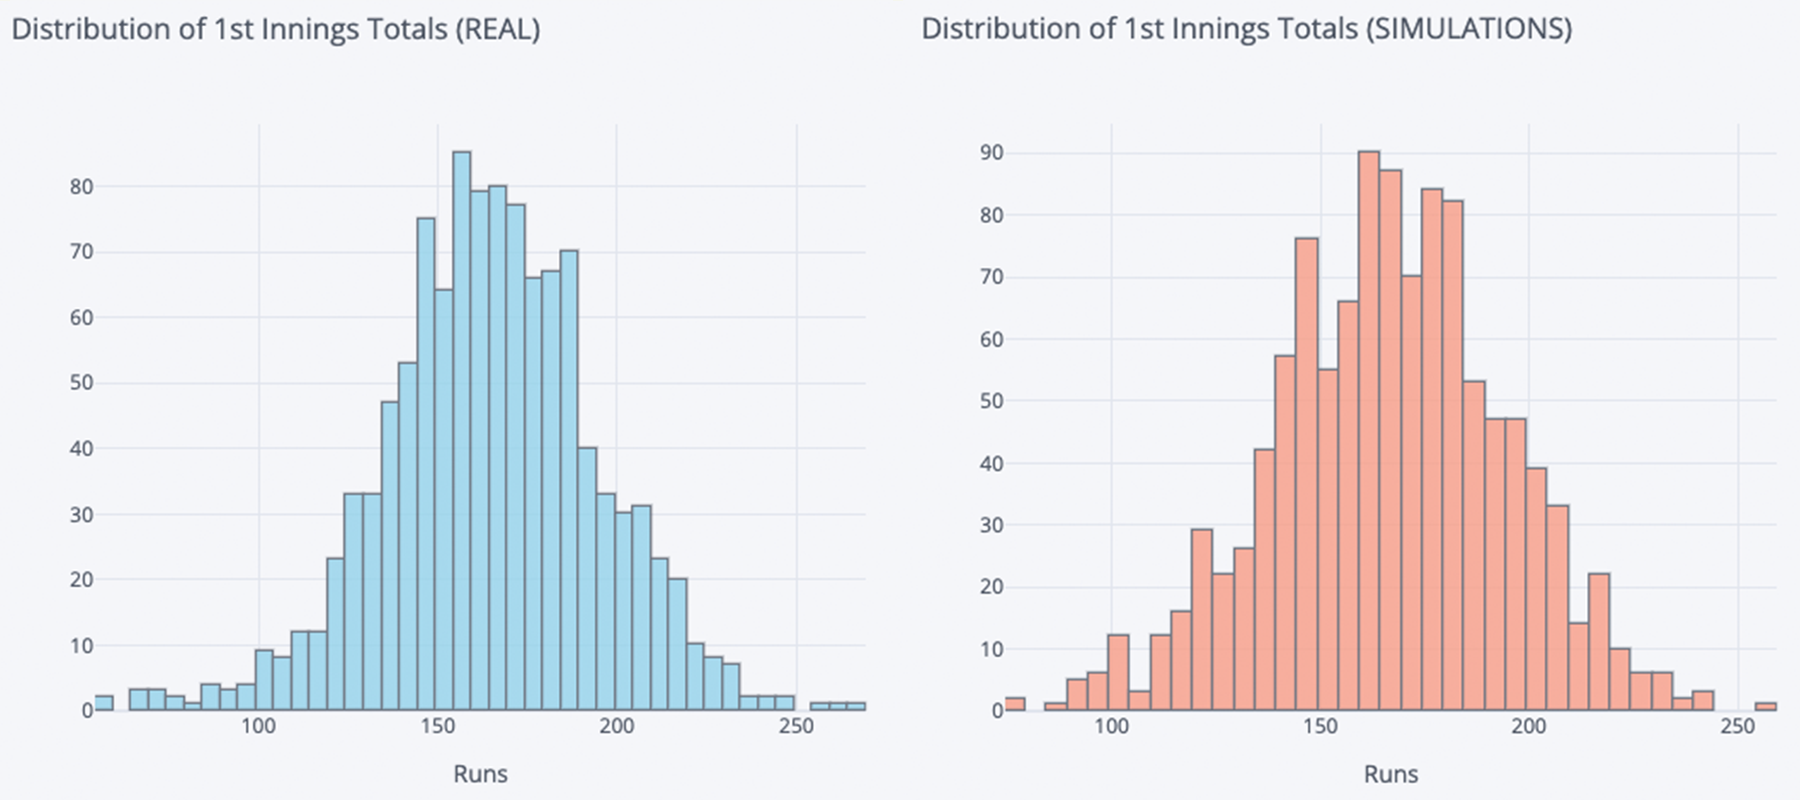
\includegraphics[width=0.7\columnwidth]{images/kuo2.png}
    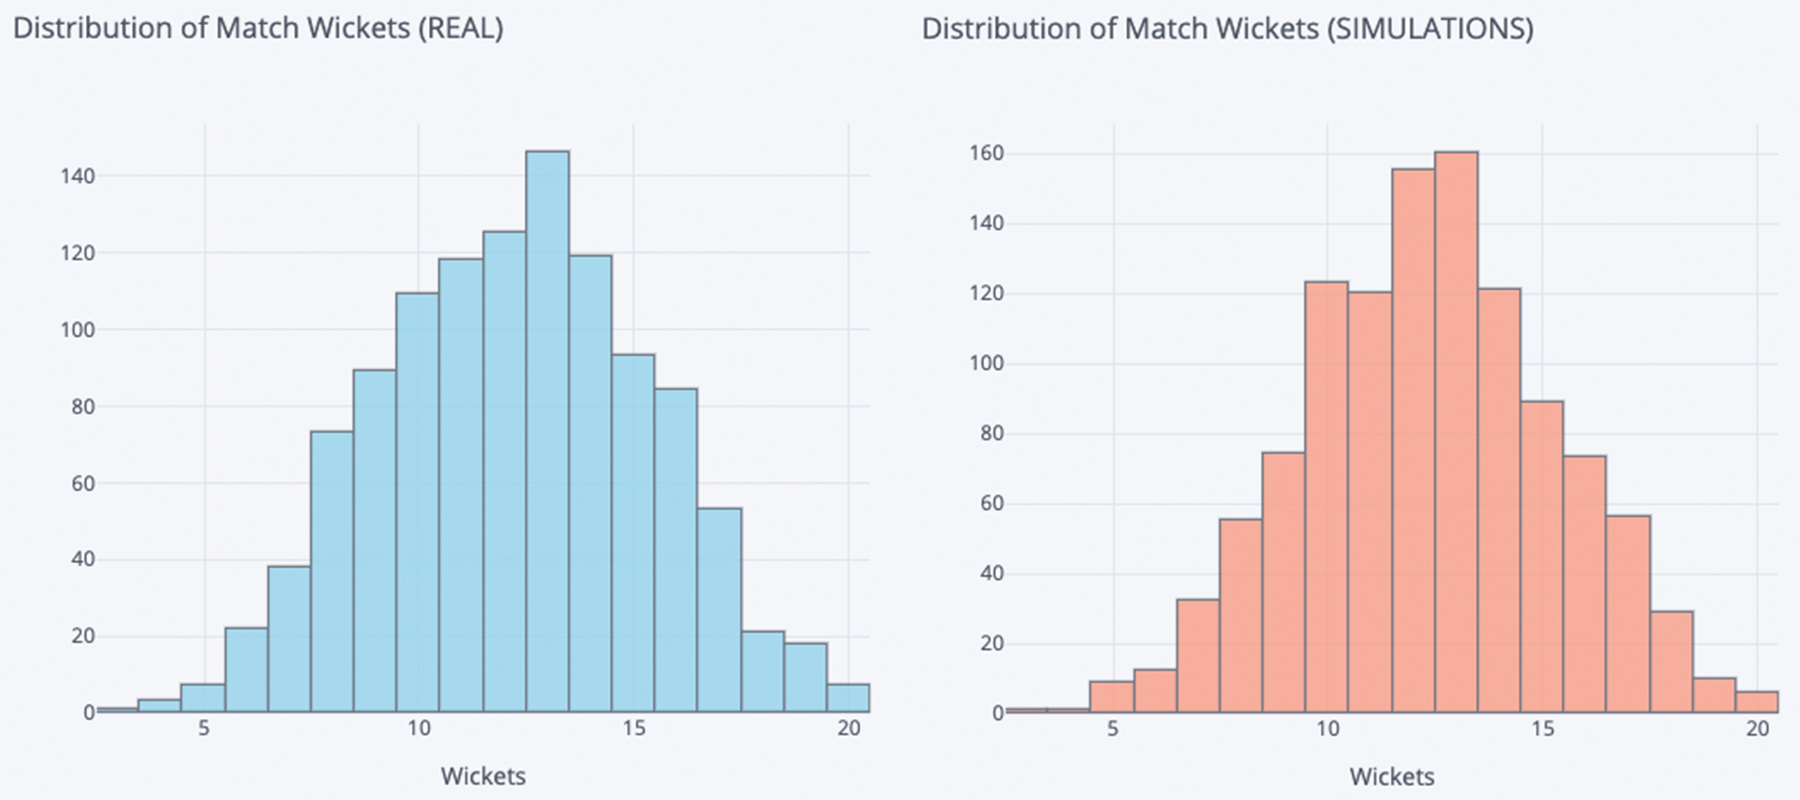
\includegraphics[width=0.7\columnwidth]{images/kuo3.png}
    \caption{Results from Kuo's simulations show a very reasonable likeness between his simulations and outcomes in real matches.}
    \label{fig:kuo2}
\end{figure}

Looking at the graphs in \cref{fig:kuo2} the conclusion was made that the simulations were a good representation of the real-life games.

A more quantitative test followed this where match outcome accuracy of the simulation model was tested. This yielded an accuracy of 55.6\%, corresponding to a log-loss figure of 0.687. When this is compared to historical betting odds from Bet365, Kuo’s model outperforms them. The bookmaker predicted the winner with an accuracy of 54.2\% and a higher log-loss score of 0.695. While encouraging, the author notes that a model with no information (i.e. guessing the winner with probability 0.5) corresponded to a log-loss of 0.693. Meaning that the Bet365 odds are less accurate than a naïve model with no information! The conclusion drawn from this is that predicting T20 match results is really rather difficult. A hypothesis is posed that accuracy could be improved if simulations were possible beyond the limit of 500.

The second part of the results looks at the model’s performance for outcomes within the game. The first test is first-innings runs. The results for which can be found in \cref{fig:kuo5}.

\begin{figure}[hb]
    \vspace{0.5em}
    \centering
    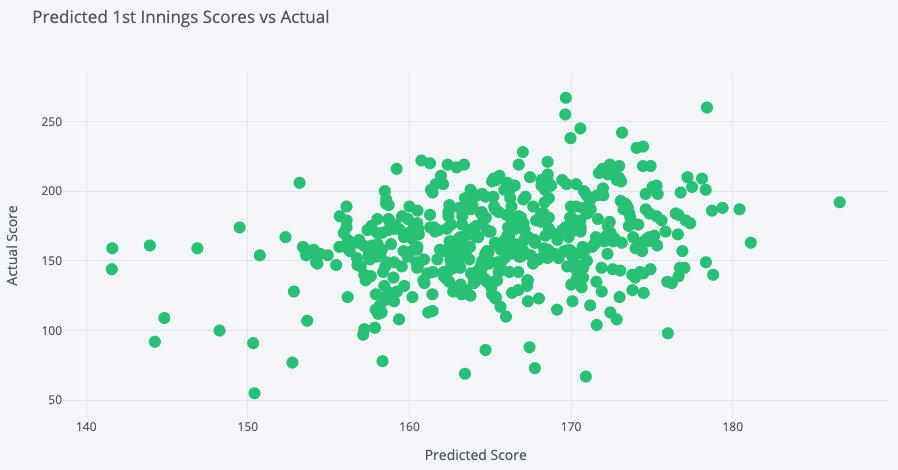
\includegraphics[width=0.9\columnwidth]{images/kuo5.png}
    \caption{Predicted first innings scores against actual first innings scores. A general trend is detectable, but it's noisy.}
    \label{fig:kuo5}
\end{figure}

The correlation between actual runs and predicted runs comes to 0.305 with a $p$-value of essentially 0. The model clearly captures the underlying factors that go into a successful prediction however the high standard deviation (28.6 runs) suggests that several other key variables are missing from the model.

The final two tests were concerned with trying to predict the top run-scorer and top wicket-taker in a given match. Kuo determines the model’s prediction for these by selecting the player who was the highest run-scorer/wicket-taker in the most simulated innings. The results were that the highest run-scorer in a given innings was predicted with around a 25\% success rate. The highest run-scorer appeared in the model’s top 4 selections on 80\% of occasions. For the highest wicket-taker, the raw success rate was 35\%. On 75\% of occasions, the highest wicket-taker in the innings appeared in the model’s top 3 selections.

\subsection{Comparing the Two Approaches}

Both papers identify the crux of this problem to be generating a probability distribution of a number of categorical outcomes. The Swartz paper uses Bayesian methods to estimate the parameters of the model, while the Kuo paper uses a neural network. Here, I outline the arguments for each of these methods and consider ways of improving upon them.

The Bayesian techniques applied by Swartz et al., are inherently stochastic, and add an extra layer of randomness and chance to the system. This is exactly what we want in a stochastic simulator. Before the model is run, each parameter input is sampled from a posterior distribution. Only then are these sampled parameters fed into the model to output the final distribution of probabilities. It’s noted in the paper how this is initial sampling is analogous to accounting for the form of the players involved in a given delivery.

The downside to this technique is the number of parameters used as inputs to the model. In this case, each of the more than 800 bowlers and batters in the dataset was assigned a parameter. This could result in the model over-fitting the data. Evidence against this suggestion was conspicuously lacking in the paper. A way in which this could be mitigated, while staying true to the underlying Bayesian principles could be to use a clustering analysis technique, to categorise the batters and bowlers into clusters, based on the similarities of their historical statistics. Some experimentation would likely be required to find the optimal number of clusters. Another advantage to this would be that the parameter values would be trained on a much wider pool of data. Rather than the model being trained on historical information for a specific bowler (who may have bowled very few deliveries in the dataset) it can consider deliveries from many more bowlers of a similar profile.

Kuo’s neural network takes far fewer parameters as inputs compared with the Swartz model. Here, batters and bowlers are not treated as factors. They are represented solely by their historical statistics. This is ideal, as the model can still use information from the entire dataset when making predictions for future outcomes. It is also the case that in a deterministic set-up like this, players with similar past statistics will be expected to perform similarly into the future which lines up with our intuition. 

We saw in the results section in \cref{fig:kuo5} that Kuo’s model succeeded in capturing the underlying features that go into predicting the score of a T20 innings, but the relationship between the predicted score and the actual score was riddled with noise. It may be that a more complex model might give predictions with greater precision and a smaller standard error. One area where significant detail can be added is in the simulation. Kuo includes 8 of the most probable outcomes but I think more scenarios could have been added. No mention is made to no-balls and the resulting free-hit, nor is any attempt made at dealing explicitly with byes and leg-byes. Improving in this area could result in increased predictive performance. Of course, it may also be the case that more variables influence these scores than Kuo or I have to model with. Weather, pitch conditions, ball conditions\footnotemark{} and many other factors, are all variables that I don’t have access to in my data that could conceivably have a significant impact on projected runs scored in an innings.

\footnotetext{By which I mean the state of the cricket ball itself, which is known to degrade over the course of a match.}

Having considered both modelling approaches carefully, I am more inclined to use Kuo’s machine learning approach for my model. One reason for this is that Bayesian computation is often extremely expensive computationally. Another is that I see inputting batters and bowlers as factors to be a significant disadvantage for reasons outlined above. For my purposes, a more classic machine learning model makes the most sense. In the next section of the literature review, I look at machine learning methods more closely and decide on a suitable one to use for my model.

\section{Machine Learning Methods}

Having decided on using a machine learning method for the main model, the next part of the literature review attempts to show how we arrived at a choice for the type of model that we'll use for this experiment.

We know that we need a machine learning tool that can handle multinomial classification. In addition to this, we require the output of the model to be a vector of probabilities, each representative of a certain outcome, which sums to 1, given each outcome is independent of all others. I choose, therefore, to investigate two methods that meet these requirements. The first is multinomial logistic regression (MLR), and the second is an artificial neural network (ANN).

\subsection{Multinomial Logistic Regression}

The short paper by Dr Jon Starkweather and Dr Amanda Kay Moske from the University of North Texas on MLR \cite{starkweather_multinomial_2011} was extremely useful to me in considering this technique's use in the model. It is essentially a primer on MLR, detailing the benefits and drawbacks of the method.

Based on Starkweather and Moske's assessment and my requirements, it seems that MLR would be an adequate tool for use in this project. However, one area of concern I have relates to a line in the article to do with training data. "Sample size guidelines for multinomial logistic regression indicate a minimum of 10 cases per independent variable." I was hoping to improve upon the Kuo model by increasing the number of output categories, which would result in some of these categories being considered very rare events, in the context of the data. I expect the model to have at least 20 inputs, which would mean I would need more than 200 instances of the rarest outcome (5 runs) in my data, which I do not have.

Another reservation I have about this method is in the construction of the model. MLR models are extensions of the generalized linear model (GLM) framework which are underpinned by the linear predictor function. Whilst this is a purposefully flexible framework, it may be the case that the inputs to my model (comprising many different variables on different scales) are unable to comfortably fit into this structure. A more flexible idea that offers similar functionality to MLR is the artificial neural network model, introduced in the following section.

\subsection{Artificial Neural Networks}

Before this project, I had no experience working with neural networks. The resources I talk about here in this section are therefore quite rudimentary, but I include them as they gave me the understanding that I now have of these systems, and enabled me to carefully evaluate their suitability for this project.

\subsubsection{3blue1brown}

The first reference is the YouTube series \cite{3blue1brown_but_2017} from the channel, \textit{3blue1brown}, created by Grant Sanderson. The series is a phenomenally well explained, comprehensive and ground-up introduction to feed-forward neural networks, with no prior experience assumed.

The series is split into four episodes. The first explains the structure of the network while walking us through the classic hand-written digits example to explain what's going on inside the network. Individual neurons are explained before the layers of the network are introduced. Then we discover how the many parameters (weights and biases) work to lead the network to output a certain prediction. Beautiful and easy-to-follow graphics accompany everything throughout the video.

Subsequent chapters get into the maths of the whole process a little more. Chapter 2 is dedicated to gradient descent - how neural networks learn. It introduces cost functions and explains how the gradient descent algorithm changes the parameters of the network to minimise this function.

\subsubsection{Ghatak}

The second reference here is a book by Abhijit Ghatak called \textit{Deep Learning with R}. \cite{ghatak_deep_2019} All of the code that we use in building and running the simulator is written in the R programming language. This book was useful as it gave me the skills to implement the principles that I learned in the Sanderson videos in the development of my own models, that can be integrated seamlessly into the simulator.

Chapter 1 of the book, an introduction to machine learning, goes through many of the basic principles of fitting machine learning models to data. The bias-variance trade-off is talked about as well as over and underfitting. It also goes through and introduces many of the hyperparameters we can decide to tweak or add to, governing the training process of the build. Chapter 3 introduced the R package Keras used for building and training neural networks, which is what we use in the main model. Chapter 6 revisits the Keras package and explains the endless tuning options available to us, how to use them and why we might want to use them. It was a vital reference book for me during the model building phase of the project.